%%
%% IIVP 2026 report template
%%
\documentclass[a4paper,fleqn]{cas-sc}

\usepackage[authoryear]{natbib}

\usepackage{float}
\usepackage{amsmath}
\usepackage{booktabs}
\usepackage{graphicx}
\usepackage{multirow}

%%%Author definitions
\def\tsc#1{\csdef{#1}{\textsc{\lowercase{#1}}\xspace}}

\begin{document}

\graphicspath{{./}}

\shorttitle{Group 9}
\shortauthors{Group 9}

\title [mode = title]{IIVP2026 Group 9 Report}

% Authors in alphabetical order by last name.
% Student IDs: digits only, no leading i/I.
\author[1]{Alexandru Cioc}[orcid=6365661]
\author[1]{V. Munoz}[orcid=6346464]
\author[1]{A. Visoiu}[orcid=9999999]

% Do not change!
\affiliation[1]{organization={Department of Advanced Computing Sciences, Maastricht University},
            city={Maastricht},
            country={The Netherlands}}

% Do not change!!
\begin{abstract}
This report has been submitted for the KEN3238 - Introduction to Image and Video Processing course in Department of Advanced Computing Sciences at Maastricht University. The report is a requirement of the IIVP-2026 challenge. The challenge has been created by Dr. Yusuf Can Semerci and Dr. Gaurvi Goyal \citep{the_challenge}.
\end{abstract}

% Do not change!!
\begin{keywords}
KEN3238 \sep IIVP2026 \sep Hindi-MNIST \sep Digit Recognition
\end{keywords}
\maketitle
\clearpage

\section{Methodology}

\subsection{Overall Approach}

Our solution is built on transfer learning using a pretrained convolutional neural network, augmented with an ensemble of independently trained models and test-time augmentation (TTA). Transfer learning has been shown to yield strong results on image classification tasks even when the source and target domains differ substantially \citep{krizhevsky2012imagenet,deng2009imagenet}, because low-level feature detectors (edges, curves, textures) learned from large-scale natural image datasets transfer effectively to handwritten character recognition.

\subsection{Model Architecture}

We adopt EfficientNet-B0 \citep{tan2019efficientnet} as the backbone. EfficientNet-B0 was designed via neural architecture search with compound scaling—jointly scaling network depth, width, and resolution by a fixed ratio—resulting in a model that achieves high accuracy with relatively few parameters compared to prior architectures. The backbone is initialised with weights pretrained on ImageNet \citep{deng2009imagenet}, providing a rich set of visual features from the outset.

The original EfficientNet-B0 classification head is replaced with a two-layer head consisting of a dropout layer with drop probability $p = 0.3$ \citep{srivastava2014dropout} followed by a linear projection from 1280 features to 10 output logits. All backbone layers are fine-tuned end-to-end; no layers are frozen during training.

\subsection{Input Preprocessing}

The dataset consists of $32 \times 32$ pixel grayscale images. To be compatible with the three-channel input expected by the ImageNet-pretrained backbone, each grayscale image is converted to a three-channel representation by replicating the single channel across all three colour channels. Images are then resized to $96 \times 96$ pixels using bilinear interpolation, and normalised using the ImageNet channel mean $\mu = (0.485, 0.456, 0.406)$ and standard deviation $\sigma = (0.229, 0.224, 0.225)$.

\begin{figure}[H]
    \centering
    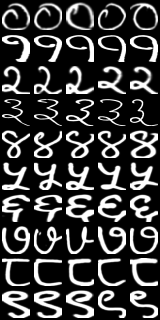
\includegraphics[width=0.85\linewidth]{Images/sample_grid.png}
    \caption{Representative samples from the training set. Each column corresponds to one of the ten classes (0--9). The characters are handwritten symbols that can appear visually similar across classes, motivating the use of strong regularisation and ensemble methods.}
    \label{fig:samples}
\end{figure}

\subsection{Data Augmentation}

During training, the following geometric augmentations are applied on-the-fly:

\begin{itemize}
    \item \textbf{Random rotation:} each image is rotated by a uniformly sampled angle in $[-15°, +15°]$.
    \item \textbf{Random affine:} random translation of up to 10\% of image dimensions and random scaling in $[0.9, 1.1]$.
    \item \textbf{Random perspective:} projective distortion with a distortion scale of 0.2 and application probability 0.5.
    \item \textbf{Random erasing:} a randomly sized rectangular patch of the image is replaced with noise, with probability 0.1 \citep{zhong2020random}.
\end{itemize}

Horizontal flipping is deliberately excluded: the handwritten symbols are not left--right symmetric, and flipping would change the visual identity of several characters, effectively corrupting the labels.

\subsection{Regularisation}

\paragraph{Mixup.} At each training step, pairs of samples $(\mathbf{x}_i, y_i)$ and $(\mathbf{x}_j, y_j)$ are drawn and combined as:
\begin{align}
    \tilde{\mathbf{x}} &= \lambda \mathbf{x}_i + (1-\lambda)\mathbf{x}_j, \\
    \tilde{y}          &= \lambda y_i + (1-\lambda) y_j,
\end{align}
where $\lambda \sim \mathrm{Beta}(\alpha, \alpha)$ with $\alpha = 0.3$ \citep{zhang2018mixup}. Mixup encourages the model to behave linearly in the space between training examples, acting as a strong regulariser.

\paragraph{Label smoothing.} Instead of training against one-hot targets, we apply label smoothing with $\varepsilon = 0.1$ \citep{muller2019label}. The target distribution is:
\begin{equation}
    \tilde{p}(k) = (1 - \varepsilon)\,\mathbf{1}[k = y] + \frac{\varepsilon}{K},
\end{equation}
where $K = 10$ is the number of classes. This prevents the model from becoming overconfident and improves calibration.

\subsection{Optimisation}

We use AdamW \citep{loshchilov2019adamw}, a variant of the Adam optimiser that decouples weight decay from the gradient update, as our optimiser. The learning rate follows a cosine annealing schedule \citep{loshchilov2017cosine} with a linear warmup over the first three epochs. The peak learning rate is set to $5 \times 10^{-4}$ and decays to approximately zero over 40 training epochs.

To accelerate training and reduce GPU memory usage, all forward and backward passes are performed in IEEE 754 half-precision (float16) using automatic mixed precision (AMP) \citep{micikevicius2018mixed}, with a GradScaler to maintain numerical stability. Gradient norms are clipped to a maximum of 1.0 to prevent training instability.

\subsection{Multi-Seed Ensemble}

Three models are trained independently using random seeds 42, 123, and 456. Each seed controls weight initialisation, batch shuffling, and stochastic augmentation, producing models that have learned complementary decision boundaries. At inference time, the softmax probability vectors from all three models are averaged element-wise:
\begin{equation}
    \hat{p}(k) = \frac{1}{M} \sum_{m=1}^{M} p_m(k), \quad M = 3,
\end{equation}
and the predicted class is $\hat{y} = \arg\max_k \hat{p}(k)$. Ensemble averaging reduces variance and improves robustness to outlier predictions from any single model.

\subsection{Test-Time Augmentation}

For each test image, five inference passes are performed: one on the original image and four on geometrically perturbed copies (rotations of $+8°$, $-8°$, $+15°$, and $-15°$). The resulting softmax distributions are averaged before combining with the ensemble. In total, each test image is processed by $3 \text{ seeds} \times 5 \text{ TTA passes} = 15$ forward passes, and the final prediction is taken as the class with the highest mean probability.

\bibliographystyle{cas-model2-names}
\bibliography{references}

\end{document}
